% COS598 Project Paper
% Authors: Aaron Doll, Shaheed Chagani, Michael Kranch, Vaidhyanath Murti
%%%%%%%%%%%%%%%%%%%%%%%%

\documentclass[10pt, letterpaper, twocolumn, twoside]{article}
%\usepackage{epstopdf}
%\usepackage[pdftex]{graphicx}
%\usepackage[left=.8in,top=.8in,right=.8in,bottom=.8in,nohead,nofoot,columnsep=20pt]{geometry}
\usepackage[left=1in,top=1in,right=1in,bottom=1in,columnsep=20pt]{geometry}
\usepackage{setspace}
\usepackage[small,compact]{titlesec}
\usepackage{subfigure}
%\usepackage{hyperref}
%\usepackage{multicol}
%\usepackage{multirow}
\usepackage{textcomp}
\usepackage{mathtools}
\usepackage{amsmath}
\usepackage[hyphens]{url}
\usepackage{float}
\usepackage{color}
%\usepackage{fancyhdr}
%\setlength{\headheight}{14.5pt}
%\setlength{\footskip}{11pt}
%\pagestyle{fancy}
%\lhead{}
%\chead{}
%\rhead{}
%\rfoot{}

\newcommand{\tab}{\hspace*{2em}}
\newcommand{\hi}[1]{\textcolor{red}{#1}}

\makeatletter
\setlength{\@fptop}{0pt}
\makeatother


%make title bold and 14 pt font (Latex default is non-bold, 16 pt)
\title{\bf btctrackr : Finding and Displaying Clusters in Bitcoin}
\author{Aaron Doll, Shaheed Chagani, Michael Kranch, and Vaidhyanath Murti\\
\textit{\{adoll, schagani, mkranch, vmurti\} @cs.princeton.edu}\\
\url{https://github.com/adoll/btctrackr}}
\date{COS 598B Privacy \\ 14 May 2014}

\begin{document}

\maketitle

% suppress page numbers
\thispagestyle{empty}

\begin{abstract}
Bitcoin is the most widely known and accepted of a rapid growing set of online, virtual crypto-currencies. Many users are attracted to these new crypto-currencies because they are decentralized and are not controlled by any authority. They are also adopting crypto-currencies because they provide pseudonymity - an individual can make online transactions with the virtual currency without any direct link to their real world identity. Because of this psuedonymity, many users believe they can use crypto-currencies freely without any risk of their transactions being traced back to their real identity; however, several recent papers on bitcoin transactions increasingly demonstrate that this belief is false. In fact, an individual's spending habits may be more easily tracked by an adversary due to the public nature of the bitcoin transaction ledger, especially when compared to more commonly accepted online payment methods like credit cards. Continuing the work presented in ``A Fistful of bitcoins'' by Meiklejohn et. al.\cite{fistfull}, this paper revisits the heuristics for identifying clusters, or the subset of bitcoin addresses likely controlled by the same entity. We then implement these heuristics in a real-time and publicly available web service. This service helps individuals identify their own linked clusters to increase privacy as well as check the recipient's address cluster prior to making a transaction to avoid addresses with possible links to theft or fraud.  
\end{abstract}

\section{Introduction}
\label{intro}
In this section, we present a brief overview of technical aspects of bitcoin. We then describe several known methods of linking bitcoin addresses presented in previous work. Finally, we discuss issues with these methods and the motivation for a real-time heuristic utility. 

\subsection{Bitcoin}
Bitcoin is an experimental, decentralized digital currency that uses peer-to-peer technology to operate with no central authority. Bitcoins are sent from one address to another with each user potentially having many, many addresses. Each payment transaction is cryptographically signed by the owner to prevent illegitimate spending and then broadcast across the peer-to-peer network to be included in the list of previous transactions (more commonly known as the block chain). Miners are special types of users that participate in the network. Miners are responsible for verifying the authenticity of an announced transaction based on the previous transactions in the block chain and including that transaction in the next block (update) to the block chain. Once a transaction is included in the block chain, that transaction can not be altered or reversed.

In the bitcoin protocol, transactions are simply a list of inputs with a corresponding list of transactions as outputs. To generate an address, a user creates a cryptographic key pair with a public and private component. The bitcoin address is an alphanumeric representation of the hash of the public key, while the private key is kept secret and is used to sign transactions to verify their authenticity. Each input is the hash of a previous transaction, as well as an index into the outputs of that transaction, and a script, which is a bitcoin specific language used for verifying transactions. Each input tuple of (transaction hash, index) is a unique reference to an output of a previous transaction. In order for a transaction to be valid, the sum of all the inputs must be greater than or equal to the sum of all the output address with the difference being claimed by the miner (an optional small fee for publishing the transaction).  Figure \ref{fig:transaction} shows an example transaction where Alice pays Bob 12 BTC. This example also shows Alice paying herself 2.9 bitcoin into what is commonly called a change address and leaving a transaction fee of 0.1 BTC.

\begin{figure}
  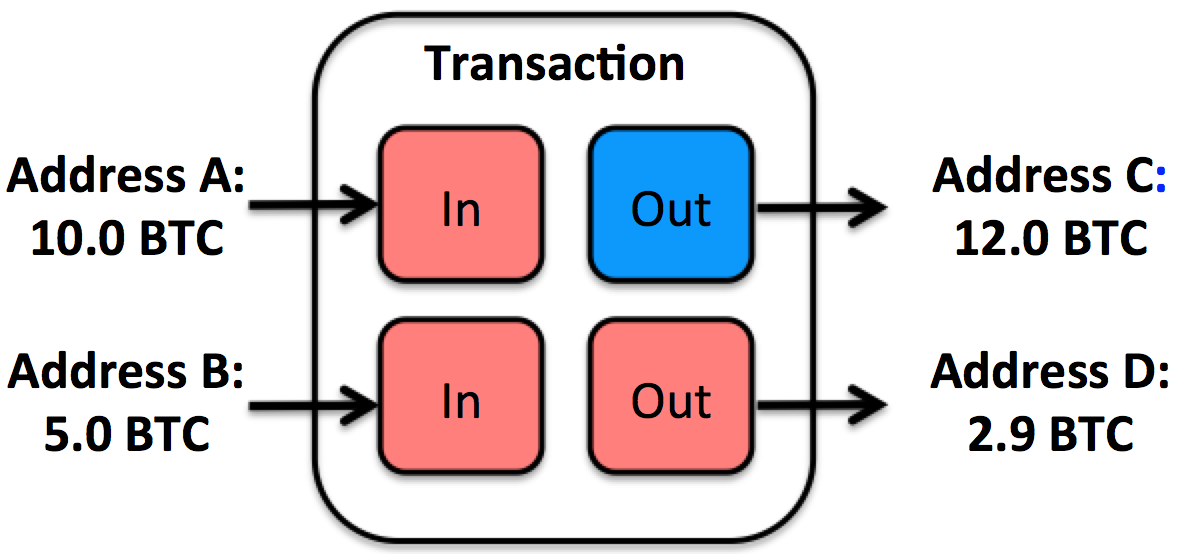
\includegraphics[width=\linewidth]{transaction2.png}
  \caption{Example Transaction}
  \label{fig:transaction}
\end{figure}

\subsection{Address Clustering}

We must first introduce some definitions to assist in our discussion of bitcoin. In traditional banking, account ``control'' is defined as the individual or set of individuals that are authorized to access to that account to transfer funds and initiate transactions. In bitcoin, we similarly define control as individual or set of individuals who can make transactions with the address through possession the address' private key.\footnote{Refer to \cite{fistfull} for a more nuanced definition of cluster and control.} Due to the nature of private keys, we also assume that the individual(s) that control an address will retain control of that address for life. 

Another concept unique to crypto-currencies is the concept of clustering. As referenced earlier, a single individual or entity might control many bitcoin addresses. The bitcoin protocol actually recommends using a new address as the outputs from every transaction to increase user privacy, and the majority of wallet applications \footnote{Wallets are bitcoin specific software systems designed to help users manage their addresses and make transactions.} default to generating a new change address in every transaction.  We will use the term cluster to mean the group (subset) of bitcoin addresses that are controlled by the same individual. In Figure \ref{fig:transaction}, Addresses A and B are both inputs to a single transaction so we can infer these addresses must both be controlled by the same individual and, therefore, belong to the same cluster. This observation leads to the very well-known method of bitcoin clustering introduced in the original bitcoin paper by Satoshi himself\cite{bitcoin} and named ``Heuristic 1'' in Meiklejohn et. al.'s paper\cite{fistfull}, 

There are several more advanced methods of clustering.  Another common method of clustering is to predict the change address from a transaction and cluster that with the inputs. In Figure \ref{fig:transaction}, Address D (the change address) is part of Alice's cluster. This heuristic is relatively fragile compared to the inputs heuristic, and aggressive implementations require large amounts of hand tuning to prevent false positives. In the early blockchain, there was a bug in the bitcoin implementation, causing change addresses to always be the first output in a transaction. This allows such addresses to be added to clusters with greater confidence and less hand tuning, but due to time constraints we did not implement this heuristic in btctrackr. Meiklejohn et. al also presented ``Heuristic 2'' as a attempt to predict the random change address, but the heuristic required significant human adjustment to avoid excessive false positives.

\subsection{Motivation}
Users of bitcoin can benefit from a tool that clusters addresses in many ways. First, users are able to monitor addresses that can be linked to them; this makes it easier for users to maintain their privacy. Second, users are able to view the clusters of people they wish to transact with which can help verify the authenticity of the addresses they are transacting with. Another tool for privacy protection is to check if one of their addresses are linked to another through a transaction between the two addresses' respective clusters. Finally, users can monitor addresses of special interest in order to estimate the total wealth of certain individuals or organizations (For example, users might wish to monitor addresses that are linked to bitcoin's founder Satoshi). While this may seem to harm the privacy of these individuals, we feel that showing the potential for this kind of discovery will raise awareness for the need to be privacy conscious even when using bitcoin. There are few public implementations of these functionalities, but most of them are inaccessible to the average bitcoin user, are slow, and as we discovered, sometimes inaccurate.


\section{Related Work}
\label{related}
The initial idea of clustering and identifying bitcoin addresses has been around since the inception of the protocol in the original bitcoin paper. As previously referenced, there are also several published papers on this topic and software implementations of these heuristics. ``A Fistful of Bitcoins'' by Meiklejohn et al\cite{fistfull} is the most notable of these papers. This work goes into great detail on the methodology of clustering heuristics and demonstrates the likability of addresses to real-life identities; however, this paper suffers from several issues. First, the results are not parsable without human intervention and, therefore, not in real time. In our discussion with Meiklejohn, she mentioned that their algorithm originally linked the majority of addresses into a single cluster and required numerous hours of link deletion by hand before achieving accurate results. As such, Meiklejohn et. al.'s software is not available for widespread use.

Znort967's Github block chain parser is another very well known implementation of Heuristic 1\cite{znort}. While freely available, this implementation requires a higher level of technical proficiency to build and run. This code is also very slow: while using the cluster module it takes over a half hour to parse the block chain and over 20gb of virtual memory. It builds an in memory graph which for every query runs a depth first search to find connected components. This software actually takes less time to parse the block chain than ours, but that is because the author trades initial computation time for additionally computation during the queries. We decided that while we could have adopted this approach, we wanted user queries to be as fast as possible.

BitIodine \cite{bitiodine} is a project out of the Politecnico di Milano\cite{bitiodine}. Spagnuolo recently published (March 2014) an additional front end web service similar to our deployment described in this paper. The BitIodine parser was built on znort967's code, and it does implement some additional change heuristics; however, his system also has several issues include downtime for block updates, slow database return calls and, most notably, a sometimes inaccurate implementation of Heuristic 1.  We suspect this is really a bug in znort987's parser, and we plan on contacting Spagnuolo to help pinpoint the issue. Basically, some transactions seem to be overlooked by the BitIodine clusters, which would be explained by the parser failing to extract the address from some inputs, or the transaction being parsed incorrectly.

Despite there being several previously published papers and applications on this topic, the lack of a readily available, accurate, real-time application of the bitcoin clustering algorithm is our motivation for this project. Our system is a real-time implementation of the Heuristics in ``A Fistful of Bitcoins''\cite{fistfull}, focusing on a clean implementation of Heuristic 1. 

\section{btctrackr}
Our system is divided into three parts: a parser, database and web frontend. We first discuss our parser, built upon the existing libbitcoin library and our implementation of cluster mapping. We then present the design of our database focusing on availability and incremental updates. Finally, we will present our front-end web service that handles user requests, queries our database and displays results to the user in an easy to use interface.

\subsection{Parser}
When designing our parser, we had two major design goals: we wanted a parser that was incremental, allowing real time updates based on the most recent blocks, and we also wanted to allow users to make nearly instantaneous queries for any address. This ruled out many of the approaches taken by others, such as that taken by Spagnuolo\cite{bitiodine} or Znort987\cite{znort}. Both of these approaches used graphs, where connected components are computed on a graph whenever a user makes a query. We decided that this was too slow, so we opted for a database-based approach, where we maintain a database that contains an address-cluster-id mapping. Since blocks are released
approximately every 10 minutes, this allows us to make use of a relatively slow incremental updater using a naive linked-list disjoint set implementation. We initially tried this approach for building the database from the block chain, but we quickly realized that this would simply be too slow. After trying a few different data structures, we settled on using a disjoint set maintained in memory, which we wrote to the database after reaching the end of the current chain. At that point we picked up with our incremental, slower database updater, which would keep our database up to date.

Initially, we were going to use a parser written by znort987\cite{znort}, but after reviewing the code we thought it looked a little unreliable, and needed some significant changes to accomplish our goals. We started exploring the different bitcoin libraries, and settled on a C++ library called libbitcoin\cite{libbitcoin}. We primarily chose this library because it looked like it had some solid community support, while also providing some very useful examples and documentation to help us get started. We were also attracted by its asynchronous event based design. We have had some difficulties due to our use of this library, but it was adequate for implementing our core functionality, with a few stumbling blocks along the way.

In order to find all addresses in a block, we iterate through all transactions in the block. For any transactions with more than one input, we attempt to obtain all the input addresses used. This was much harder than we expected, due to what we have assumed to be some irregularities with earlier versions of the bitcoin protocol. In our description of a bitcoin transaction, you may have noticed we made no mention of the addresses of either inputs or outputs. That is because the address is actually contained within the bitcoin script of each input or output. While this seems to be always true for output scripts, we discovered that relying on input scripts containing the address resulted in numerous missing addresses, especially early in the block chain. We aren't sure whether this was a problem with libbitcoin's function for extracting addresses from script or simply the fact it is in an ill-defined format, although we conjecture that this is due to a lack of standardized scripts in the protocol at that time. Fortunately there is another way to get the address, since each input tuple (transaction\_hash, index) uniquely defines an output point of a previous transaction, we can fetch that transaction and extract the address from that output's script.

This error was in fact related to our biggest problem with libbitcoin: when trying to expand our core functionality, we ran into occasional correctness problems. While adding balances for each address, we discovered that some of libbitcoin's functions were simply wrong. We narrowed the problem down to the fact that some addresses were missing transactions, specifically spends, which led to massively inflated address balances. After further investigation, we discovered that the problem was the same problem we had in the parser, extracting the input addresses from the script was failing in one of their core files for parsing the block chain, causing these spends to be left out of queries for the history of specific addresses. We fixed the problem in much the same way as we did in our parser, but unfortunately we found there are still transactions missing for select addresses (although much fewer than before). While this doesn't affect our core clustering functionality, it does lead to problems when checking for 1-hop paths between addresses, causing potential false negatives. By the time we discovered this bug, we had already downloaded the block chain again in order to implement our simple fix (the problem code runs as each block is added to the blockchain database), so we didn't have time to investigate further causes of this bug.

Another disadvantage to libbitcoin we discovered is that it is memory-hungry. If we tried to process the whole blockchain at once (as encouraged by their stateless, event-based asynchronous library), it consumed an excessive amount of RAM. Instead, we had to introduce state so that only 10,000 were processed at once, which seems to run counter to the ideas behind libbitcoin. We felt their library should have some kind of limit on the number of blocks open at once, and then it would simply queue your requests, rather than silently choking yor system.

\subsection{Database}

After we decided to choose the database approach, we were faced with the decision of choosing an efficient and fast database. We settled on using MySQL for two reasons: First, SQL databases are optimized for queries which tied in well with our goal of providing a fast website. Second, MySQL was easy to connect with both the backend and front-end of our project. We used a simple schema that involved one table with an address as the primary key and an integer that represented the cluster. This set up allowed us to easily insert address-cluster mappings when they were computed by our parser and retrieve the cluster for an address when it was requested by our website. Using MySQL was not without its limitations; it proved to be much slower than we expected while inserting into the database leading to large build cycles. The database insert phase was always the bottleneck in our development cycle, especially given the size of the block chain.

BitIodine, another implementation of this facility, described his setup with 4 separate databases. One holds the block chain, another has the transaction graph, another database contains the balances and other features, and the final one for trades. While this setup might provide more insight into the block chain, we felt that adding more complexity to our setup would result in a increased latency to the website which conflicted with our initial design goals. To minimalize latency, we chose to use just two databases, one fast and lightweight LevelDB database (used by libbitcoin) to hold the block chain and the MySQL database described above to hold the clusters. We feel that this approach worked well for our purposes while also providing flexibility to add additional features if desired in the future.

\subsection{Website}
We designed our web interface with two main goals in mind: we wanted to allow users to ``track'' an address and view detailed information about it, such as which other addresses likely belong to the same entity. Also, we wanted to allow users to enter in two addresses, and see if the clusters containing the two addresses are linked by a transaction. We built our website, www.btctrackr.com, with these goals in mind, and emphasized a simple, clean, easy-to-use design.

Upon visiting our website, the track feature is automatically loaded, in which a user can enter an address and press ``Track''. We send an AJAX request to our server, which looks up the $cluster\_id$ of the address in our database, and then retrieves all of the addresses corresponding to that $cluster\_id$. There are a number of front-end and back-end checks in place to ensure the user has a valid bitcoin address. On the client side, we make sure the address is a valid number of characters. On the server side, if the address is not present in our database, we query the blockr.io API to check if the address has ever appeared in a transaction, whether or not it is valid. If it is not valid, we alert our users accordingly.

We also wanted to display the current balance of each of the addresses as well as the total balance of the entire cluster. Due to problems with the libbitcoin library, we chose to leverage the blockr.io API, which has up-to-date balance information. One challenge we faced, however, is that querying a web API for several balances is significantly slower than querying a local database. Some of our clusters have hundreds or even thousands of addresses. As such, making this many API calls would lead to a tremendous delay in response time for the users. Our goal was to make our interface as responsive as possible. The blockr.io API allows clients to get balance information for up to 20 addresses in one call. To spend up our response time,  we group the addresses them into sets of 20 or less after retrieving all of the cluster addresses from the database. We then utilize $curl\_multi\_init()$ (through the parallelcurl Github library) to send off all of these API calls simultaneously, and process the results asynchronously. We found that we were able to return results to the user way faster than if we used any other method. For example, we are able to return over 100 balances in less than 1 second. However, we noticed that if we attempt to load the balances of exceedingly large clusters (thousands of addresses), the response from the server is slow, or times out. The bottleneck here is that we need to call the blockr.io API in order to retrieve balances, and we can only do so in chunks of 20 addresses. We are currently looking into devising a better solution for displaying the balances of massive clusters. In general, the user interface is very responsive, which makes our tool easy to use.

The other main feature we implemented was to allow users to enter in two addresses, and see if the clusters containing those addresses are linked by a 1-hop path. Users can enter in a source address and a destination address, and we fire off another AJAX request to our server. On the back-end, we execute a binary file that determines whether or not the two addresses are linked by a 1-hop path. On the front-end, we display the transaction hash in which an address in the same cluster as the source address transacts with an address in the same cluster as the destination address. Additionally, we display the two addresses that are part of the physical transaction. All in all, this is a quick and easy tool that allows users to find out if and how certain addresses are connected.

\section{Evaluation}

Since there is no publicly available data on clusters and it would not be feasible to manually find clusters in the block chain, we decided to evaluate our code by comparing it to BitIodine. To perform this comparison, we chose 20 random addresses and ran them through both our clustering tools. In this context, the results are summarized in the table below. We define a false positive as an address that should not be in a cluster but is (ie all addresses are not controlled by the same person), and a false negative as an address that should be in a cluster but isn't. If an address was in BitIodine's cluster but not ours, or vice versa, we considered that a false negative.

\begin{table}[h]
\caption{Evaluation of btctrackr and BitIodine}
\centering
\begin{tabular}{lc}
\hline
Tool & False Negative \\
\hline\hline
btctrackr & 35.8\% \\
BitIodine & 54.2\% \\
\end{tabular}
\end{table}

Because we do not have an established ground truth, we cannot evaluate the false positive results of these projects. However, we make the argument that our implementation should not have false positives since the heuristic it uses is guaranteed to be correct. By the definition of control over a cluster, any entity that can sign a transaction with multiple inputs necessarily controls the private keys of all the inputs in that transaction. BitIodine on the other hand implements a change heuristic that takes into account a bug in the implementation of a popular bitcoin client. While many users of bitcoin used this client it was not 100\% of the users. This means BitIodine might have classified a few of the addresses incorrectly. If our heuristic doesn't lead to false positives, then all that needs to be verified is that our implementation of that heuristic is correct. In the process of determining the ideal data structure for parsing the block chain, we compared each of 3 independent implementations and got the same results, so we are fairly confident our implementation is correct.

With regards to the false negatives, there are a few reasons why we could have them. First, at the time of testing, we had only 200,000 blocks downloaded and parsed while BitIodine had the entire block chain. Also, due to the limitations of libbitcoin, we were not able to parse multi-signature transactions and other non-standard types of transactions. Lastly, since we do not implement a change heuristic, we miss some cluster mappings that BitIodine has. On the other hand, we conjecture that BitIodine's high false negative percentage is mainly due to problems with their parser. This causes transactions to be missed that could potentially merge clusters that are others left disjoint. An example of such a transaction is the following one: a8ca4c0ba498fb5de54451b5c5b5c831535e510298c5a5
9b5fdb5b0cf86376fb. It appears as though BitIodine ignores this transaction completely as it does not merge the clusters of the addresses that are inputs to this transaction. According to BitIodine the address 15iGN5CAkTarcoY85XxwTYWajJyz5hxbYv has 13 addresses in its cluster and the address 1EKpJjAcAEe4RL5Qey4wHgsXGFZUxnD72A has 926 addresses in its cluster. If Bitiodine was able to merge this cluster and recursively merge clusters for all transactions that it missed, it would be able to grow its cluster significantly. At 200,000 parsed blocks, these addresses were in a cluster of 13,289 addresses.

\section{Conclusion and Future Work}
Overall, we were pleased with the results of our efforts, and created a relatively fast, incremental, and easy to use web interface for the clustering heuristic. That being said, there are a few problems with our current project. First of all, balances and database loads for large clusters are still slower than we'd like. In order to help speed things up, we currently don't show the balances for clusters with more than 500 addresses in it. 

Some of the limitations of our project are due to our use of libbitcoin\cite{libbitcoin}. Libbitcoin does not support multi-signature transactions as of yet, limiting the transactions we include in our cluster calculations. As we mentioned earlier, we have noticed some missing transactions, leading to potential false negatives when we check for one hop links between clusters. This may be a bigger problem than we originally thought, but is something that will be fixed with a patch to libbitcoin. We hope that this is related to the earlier problem and primarily happens for early addresses, but since we wouldn't be able to update our data at this point even if we do find the bug, we have left this for a future date. 

There are also a number of features that we simply couldn't include due to time constraints. In ``A Fistful of Bitcoins''\cite{fistfull}, the authors associate clusters with entities and graph the largest entities. We wanted to include the ability for users to submit labels to addresses, hopefully mapping the bitcoin network in detail, as well as including addresses that we labeled ourselves. In our first conception of this project, we also hoped to implement the change address heuristic, but after speaking with Meiklejohn, we decided that was not a realistic goal for a semester long project. Implementing a limited change heuristic based on the bug in early bitcoin is definitely possible, and something worth considering for the future.


% Imports the bibliography, don't remove
\small{
\begin{thebibliography}{99}

\bibitem{libbitcoin} Maersk, N., Strateman, P., Taaki, A., and Williamson, R., ``libbitcoin - Asynchronous C++ Bitcoin library'', \emph{GitHub Repository,} 2013,
\url{http://libbitcoin.dyne.org/}.

\bibitem{fistfull} Meiklejohn, S., Pomarole, M., Jordan, G., Levchenko, K., McCoy,
D., Voelker, G. M., and Savage, S., ``A Fistful of Bitcoins: Characterizing Payments Among
Men with No Names,'' in \emph{Proceedings of the 2013 Internet Measurement Conference,} 2013, \url{http://cseweb.ucsd.edu/~smeiklejohn/files/imc13.pdf}.

\bibitem{bitcoin} Nakamoto, Satoshi, ``Bitcoin: A Peer-to-Peer Electronic Cash System,'' (2008) \url{https://bitcoin.org/bitcoin.pdf}.

\bibitem{bitiodine} Spagnuolo, Michele, ``BitIodine: Extracting Intelligence from the Bitcoin Network (Master's Thesis),' 2013, \url{https://bitiodine.net/}. 

\bibitem{znort} Znort987, ``Block Parser'', \emph{GitHub Repository,} 2012,
\url{https://github.com/znort987/blockparser}.



%P.W.D. Charles, Project Title, (2013), GitHub repository, https://github.com/charlespwd/project-title

\end{thebibliography}
}
%Bit Iodine - \cite{bitiodine}
%Fistful of bitcoins - \cite{fistful}
%Satoshi - \cite{bitcoin}
%Znort987 - \cite{znort}
%libbitcoin - \cite{libbitcoin}


\end{document}
